\documentclass[12pt, twoside]{article}
\usepackage[letterpaper, margin=1in, headsep=0.5in]{geometry}
\usepackage[english]{babel}
\usepackage[utf8]{inputenc}
\usepackage{amsmath}
\usepackage{amsfonts}
\usepackage{amssymb}
\usepackage{tikz}
\usepackage{yhmath}
\usetikzlibrary{quotes, angles}
\usepackage{graphicx}
\usepackage{enumitem}
\usepackage{multicol}

\newif\ifmeta
\metatrue %print standards and topics tags

\title{Regents Geometry}
\author{Chris Huson}
\date{April 2022}

\usepackage{fancyhdr}
\pagestyle{fancy}
\fancyhf{}
\renewcommand{\headrulewidth}{0pt} % disable the underline of the header
\raggedbottom

\fancyhead[LE]{\thepage}
\fancyhead[RO]{\thepage \\ Name: \hspace{4cm} \,\\}
\fancyhead[LO]{BECA / Dr. Huson / Geometry\\* Unit 10: Trigonometry\\* 12 April 2022}

\begin{document}
\subsubsection*{10.7 Trigonometric identities \hfill HSG.SRT.C.8}
\begin{enumerate}
\item Given right $\triangle ABC$ with $AC=5, BC=5 \sqrt{3}, AB=10$, $m\angle C=90^\circ$. Express each trig ratio as a fraction, then as a decimal to the nearest thousandth. (1a is an example)
  \begin{multicols}{2}
    \begin{enumerate}[itemsep=0.2cm]
      \item $\sin A =$
      \item $\cos A =$
      \item $\sin B =$
      \item $m\angle A=$
    \end{enumerate}
    \begin{center}
      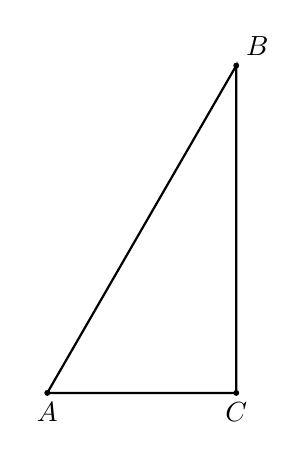
\begin{tikzpicture}[scale=0.6]
        \draw [thick](0,0)--(4,0)--(60:8)--(0,0);
        \draw [fill] (0,0) circle [radius=0.05] node[below]{$A$};
        \draw [fill] (4,0) circle [radius=0.05] node[below]{$C$};
        \draw [fill] (60:8) circle [radius=0.05] node[above right]{$B$};
        %\draw [color=blue] (0,0) ++(0.75,0) arc [start angle=0, end angle=70, radius=0.75];
        %\draw [color=blue] (4,0) ++(-0.22, 0.73) arc [start angle=110, end angle=180, radius=0.75];
        %\draw [thick] (0.8,3.1)--(1.2,2.9); %tick mark
        %\draw [thick] (2.8,2.9)--(3.2,3.1); %tick mark
        %\node [right] at (3.25,2.5){$x+7$};
        %\node [left] at (0.75,2.5){$2x+1$};
      \end{tikzpicture}
    \end{center}
  \end{multicols} \vspace{1cm}

\item Right triangle $\triangle ABC$ is shown with base $AC=6$ and hypotenuse $AB=10$ as marked.\vspace{0.25cm}
\begin{multicols}{2}
  \begin{enumerate}[itemsep=0.5cm]
    \item Write down $\cos A$.
    \item Find the length of side $BC$.\vspace{1.5cm}
    \item Write down $\tan A$.
    \item Write down $\sin A$.
    \item Find the angle measures of $\angle A$ and $\angle B$.
    \vspace{1cm}
  \end{enumerate}
\begin{flushright}
        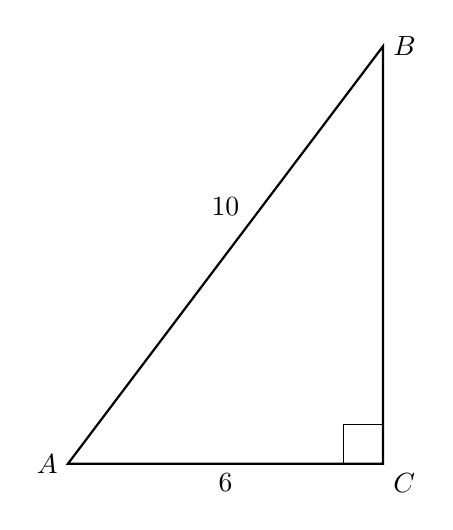
\begin{tikzpicture}[scale=1]
        \draw [thick]
        (0,0)node[left]{$A$}--
        (4,0)node[below right]{$C$}--
        (4,5.3)node[right]{$B$}--cycle;
        \draw (4,0)++(-0.5,0)--++(0,0.5)--+(0.5,0);
        \node at (2,0)[below]{$6$};
        \node at (2,3.5)[below]{$10$};
        %\node at (4,2.7)[right]{$8$};
        %\node at (1.8,2.6)[above]{$10$};
      \end{tikzpicture}
\end{flushright}
\end{multicols} \vspace{1.5cm}

\item Are the lines parallel, perpendicular, or neither? Justify your answer. \\(you must use the values of the slopes in your justification)
  \begin{multicols}{2}
    $y = 4x+1$ \\
    $y = \frac{1}{4}x-4$
  \end{multicols}

\newpage
\item Given $P(4,7)$ and $Q(5,0)$, find the length of $\overline{PQ}$, expressed as a simplified radical.\\[0.25cm]
Use: $l=\sqrt{(x_2-x_1)^2+(y_2-y_1)^2}$
    \vspace{5cm}

\item A translation $T_{x,y}$ maps $A(-1,12) \rightarrow A'(5,-2)$. 
\begin{enumerate}
  \item Write down the translation. \vspace{1cm}
  \item Apply the same translation to $B(-3, 8)$.
\end{enumerate} \vspace{1.5cm}

\item In the diagram below, $\overline{PQ}$ has endpoints with coordinates $P(-2,5)$ and $Q(4,-1)$. Find the equation of the perpendicular bisector of $\overline{PQ}$ and plot it on the grid.
  \begin{flushright}
    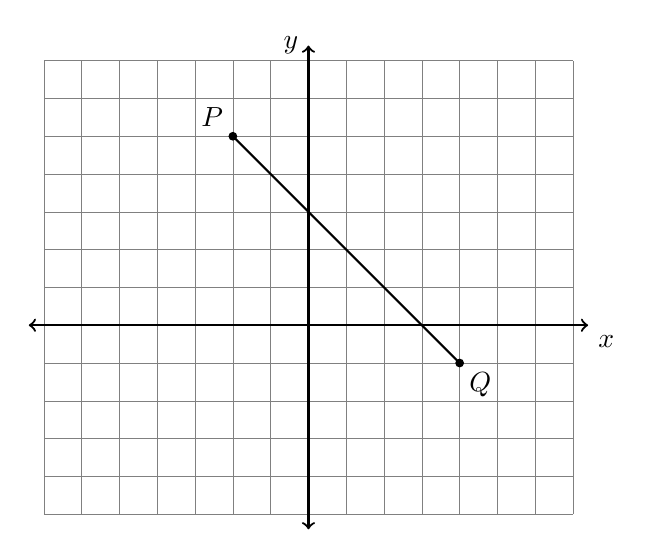
\begin{tikzpicture}[scale=.48]
      \draw [help lines] (-7,-5) grid (7,7);
      \draw [thick, <->] (-7.4,0) -- (7.4,0) node [below right] {$x$};
      \draw [thick, <->] (0,-5.4)--(0,7.4) node [left] {$y$};
      \draw [thick] (-2,5)--(4,-1);
      \draw [fill] (-2,5) circle [radius=0.1] node[above left] {$P$};
      \draw [fill] (4, -1) circle [radius=0.1] node[below right] {$Q$};
    \end{tikzpicture}
  \end{flushright}

\end{enumerate}
\end{document}
  